\documentclass[11pt,a4paper]{article}
\usepackage[utf8]{inputenc}
\usepackage{geometry}
\usepackage{graphicx}
\usepackage{array}
\usepackage{booktabs}
\usepackage{longtable}
\usepackage{fancyhdr}
\usepackage{listings}
\usepackage{xcolor}
\usepackage{enumitem}
\usepackage{hyperref}
\usepackage{tabularx}
\usepackage{amssymb}
\usepackage{amsmath}
\usepackage{tikz}
\usetikzlibrary{shapes,arrows,positioning,calc}

% Page layout settings
\geometry{left=1in,right=1in,bottom=1in,top=1.02in,headheight=46pt,headsep=0.45cm}
\setlength{\parindent}{0pt}
\setlength{\parskip}{0.5em}

% Graphics path setting
\graphicspath{{../images/}}

% Listings settings for code blocks
\lstset{
    basicstyle=\ttfamily\small,
    breaklines=true,
    frame=single,
    backgroundcolor=\color{gray!10},
    xleftmargin=0.5cm,
    xrightmargin=0.5cm,
    aboveskip=1em,
    belowskip=1em,
    columns=flexible,
    keepspaces=true,
    showstringspaces=false
}

% Header and footer setup
\pagestyle{fancy}
\fancyhead{}
\fancyfoot{}

% Define header content
\fancyhead[L]{thermal-core: Protocol-Agnostic Thermal Control}
\fancyhead[R]{\raisebox{0.05cm}{
\includegraphics[width=1.35cm]{logo.png}}}

% Define footer content
\fancyfoot[C]{\thepage}
\fancyfoot[L]{Draft 0.1 -- May 2026}
\fancyfoot[R]{}

% Header/footer lines
\renewcommand{\headrulewidth}{0.4pt}
\renewcommand{\footrulewidth}{0.4pt}

% Hyperref settings
\hypersetup{
    colorlinks=true,
    linkcolor=black,
    urlcolor=blue,
    pdftitle={thermal-core: Protocol-Agnostic Thermal Control Design \& Implementation},
    pdfauthor={Albert David}
}

% Custom colors for zones and elements
\definecolor{nightzone}{RGB}{100,150,255}
\definecolor{indoorzone}{RGB}{100,200,100}
\definecolor{outdoorzone}{RGB}{255,180,50}
\definecolor{codeblock}{RGB}{240,240,240}

%------------------------
% Document starts here
%------------------------
\begin{document}
\thispagestyle{fancy}

\vspace*{3cm}

\begin{center}
    {\huge\bfseries thermal-core}\\[1ex]
    {\Large Protocol-Agnostic Thermal Control}\\[0.5ex]
    {\Large Design \& Implementation}\\[2ex]
    {\large Author: Albert David}\\[2ex]
    {\large Draft 0.1}\\[1ex]
    May 2026\\[2ex]
    {\normalsize A Technical Guide for Portable Automotive IVI Thermal Control}
\end{center}
\vspace{2em}

\section*{Document Revision History}
\begin{longtable}{|p{0.12\textwidth}|p{0.18\textwidth}|p{0.15\textwidth}|p{0.45\textwidth}|}
    \hline
    \textbf{Version} & \textbf{Date} & \textbf{Author} & \textbf{Description} \\
    \hline
    0.1 & May 2026 & Albert David & Initial thermal-core migration from the ALS-Dimmer technical-document template \\
    \hline
\end{longtable}

\section*{Abstract}

\texttt{thermal-core} is a protocol-agnostic thermal-control core with an automotive IVI reference application. It separates deterministic control policy from platform I/O so the same zone, governor, fault, and policy logic can run on Linux, ESP-IDF, and future MCU targets. The first reference policy demonstrates acoustic-aware fan control using vehicle speed as a reproducible context signal.

This draft is intentionally a scaffold. It captures the paper structure, terminology, and fill-in points before the implementation and benchmark data are complete.

\section*{Draft Status}

\begin{itemize}[leftmargin=*]
    \item Replace scaffold text with implementation details as modules land.
    \item Add plots generated from scenario CSV files.
    \item Add commit SHAs to every benchmark table and figure caption.
    \item Keep protocol-specific details in platform/tooling sections, not in the core architecture.
\end{itemize}

\clearpage

\tableofcontents

\clearpage

%------------------------
% Part I: Fundamentals
%------------------------
\part{Fundamentals of Acoustic-Aware Thermal Control}

\section{Introduction}

\subsection{Problem Statement}

Automotive IVI systems increasingly combine high-performance SoCs, amplifiers, tuners, displays, and peripheral controllers inside compact spaces with limited passive airflow. Active cooling is often necessary, but fan noise that disappears at highway speed can become objectionable when the vehicle is stopped in a quiet cabin.

\texttt{thermal-core} explores a small, portable thermal-control core that treats cooling and acoustic comfort as coupled requirements. The first reference application is IVI fan control, but the core itself remains protocol-agnostic: it consumes typed temperature, actuator, and context signals rather than parsing Linux sysfs paths, CAN frames, OBD-II messages, or JSON directly.

\subsection{Concept Summary}

The project separates the problem into three layers:

\begin{itemize}[leftmargin=*]
    \item \textbf{Core:} deterministic C99 logic for zones, trips, governors, policy modifiers, arbitration, fault detection, and numeric telemetry.
    \item \textbf{Platform layer:} Linux, ESP-IDF, and future RH850 bindings for sensors, fans, timing, logging, telemetry, and configuration loading.
    \item \textbf{Scenario and bench tooling:} host-side tools, scripted tests, OBD-II speed emulation, data capture, and plot generation.
\end{itemize}

\subsection{Expected Contributions}

This paper will eventually document a reusable thermal-control architecture, a vehicle-speed-aware acoustic policy, a reproducible bench/HIL workflow, and measured behavior from scripted scenarios.

\subsection{To Fill In Later}

\begin{itemize}[leftmargin=*]
    \item final implementation SHA and release tag;
    \item tested host and embedded target versions;
    \item reference bench photograph;
    \item headline benchmark table;
    \item one-paragraph summary of the most important result.
\end{itemize}

\endinput

\section{Thermal Operating Environments}

\subsection{Automotive IVI Thermal Context}

The reference system is an IVI head unit operating across cabin temperature, solar loading, enclosure heat soak, and vehicle-speed regimes. The thermal controller must handle both slow heat accumulation and abrupt workload changes while preserving a clear safety order: policy may spend thermal margin, but critical cooling wins over comfort policy.

\subsection{Operating Regimes}

\begin{table}[h]
\centering
\begin{tabular}{p{0.22\textwidth}p{0.22\textwidth}p{0.42\textwidth}}
\toprule
\textbf{Regime} & \textbf{Example} & \textbf{Control implication} \\
\midrule
Parked heat soak & hot cabin, no road noise & policy modifier may cap actuator output while margin exists; fallback must fail toward cooling \\
Idle / stop light & vehicle speed near zero & avoid sudden actuator cycling; dwell and slew shape transitions \\
Urban driving & 10--50 km/h & context policy may relax caps gradually as operating context changes \\
Highway driving & 80+ km/h & context policy may permit earlier or stronger cooling while safety ordering stays unchanged \\
Fault / degraded sensor & missing tach, stale sensor, lost CAN & enter explicit fail-safe behavior and log numeric events \\
\bottomrule
\end{tabular}
\caption{Initial operating regimes for the IVI reference application. The acoustic-aware policy in Section~\ref{sec:reference-policy} is one configured modifier instance of these more general rules.}
\label{tab:thermal-operating-regimes}
\end{table}

\subsection{Reference Bench Setup}

The bench rig used for the hardware-in-the-loop bring-up (Section~\ref{sec:evaluation}) is deliberately minimal and open-air, so the setup is reproducible without an environmental chamber:

\begin{itemize}[leftmargin=*]
    \item \textbf{Controller:} an ESP32-C3 SuperMini board, USB-powered, running the reference ESP-IDF firmware.
    \item \textbf{Actuator:} a Noctua NF-A8 four-pin PWM fan driven at 25\,kHz, powered from the 5\,V USB rail.
    \item \textbf{Sensor:} a DS18B20 digital probe on a shared 1-Wire bus with a 4.7\,k$\Omega$ pull-up; additional probes drop onto the same bus.
    \item \textbf{Enclosure:} none --- the components sit on an open breadboard. During bring-up, thermal input is applied by hand (finger contact, warm air), not by a controlled heater.
\end{itemize}

Controlled per-run ambient temperature, a calibrated heat source, and a documented \texttt{car-can-emulator} speed profile belong to the formal benchmark sweep and are not yet captured.

\endinput

\section{Reference Policy Application: Acoustic-Aware Fan Control}\label{sec:reference-policy}

\subsection{Motivation}

Thermal controllers often optimize only temperature margin. In a vehicle cabin, the user-visible quality problem is more nuanced: the same fan command can feel silent while driving and distracting while stationary. A fan that disappears acoustically at highway speed can feel sudden and intrusive at a red light, even if its duty cycle changed only modestly.

\texttt{thermal-core} models this as a reference policy modifier rather than embedding cabin assumptions into the governor. The governor still computes thermal demand; the \texttt{acoustic\_mask} modifier uses vehicle speed to choose how much non-critical fan duty may be capped and whether trips should shift earlier when the cabin noise floor is higher.

\subsection{Vehicle Speed as Context}

Vehicle speed is used as the first acoustic-context proxy because it is easy to reproduce on a bench and broadly correlated with road and wind noise. The v1 reference implementation uses OBD-II PID \texttt{0x0D} only as a reproducible test source; production systems would normally use an OEM-private CAN signal or another vehicle-state service. If the speed source is stale, the reference modifier uses an explicit fail-safe mode: either hold the last valid value or assume stationary operation.

\subsection{Acoustic-Mask Curve}

The reference policy maps vehicle speed to a PWM cap and optional trip offset:

\begin{table}[h]
\centering
\begin{tabular}{ccc}
\toprule
\textbf{Speed (km/h)} & \textbf{PWM cap} & \textbf{Trip offset (m$^\circ$C)} \\
\midrule
0 & 120 & 0 \\
30 & 180 & 0 \\
80 & 255 & -5000 \\
130 & 255 & -8000 \\
\bottomrule
\end{tabular}
\caption{Initial acoustic-mask curve from the PRD. Values are placeholders until tuned.}
\label{tab:acoustic-mask-curve}
\end{table}

The cap is skipped for actuators driven by \texttt{CRITICAL} or \texttt{SHUTDOWN} zones, and spin-up is allowed to exceed the cap during its configured boost window. Modifier validation bounds both the cap and the trip offset, so this reference curve cannot silently reorder trips or ask for a non-zero PWM below an actuator's configured minimum.

\subsection{Acoustic Proxy}

Until calibrated sound-pressure measurements are available, the paper uses fan PWM-seconds and fan RPM-seconds as acoustic proxies:

\begin{equation}
    A_{pwm} = \sum_{k=0}^{N-1} PWM_k \Delta t
\end{equation}

These proxies are not a substitute for SPL data. They are useful only as reproducible scenario metrics until the formal acoustic sweep is run.

\subsection{Scenario Coverage}

The canonical scenarios \texttt{acoustic\_mask\_low\_speed.scn} and \texttt{acoustic\_mask\_high\_speed.scn} exercise the two ends of the modifier curve with a virtual CAN speed source; \texttt{can\_bus\_loss.scn} exercises the stale-context fail-safe path. These scenario names keep the original policy label, but they are tests of the generic modifier and stale-context machinery described in Section~\ref{sec:control-model}.

\subsection{Pending Acoustic Characterization}

The acoustic side of the design is documented but not yet measured. The following await the calibrated benchmark sweep on instrumented hardware:

\begin{itemize}[leftmargin=*]
    \item measured or estimated cabin-noise values for idle, urban, and highway regimes;
    \item justification for selected speed breakpoints;
    \item comparison of PWM-seconds with and without acoustic masking;
    \item a calibrated sound-pressure-level (SPL) measurement plan.
\end{itemize}

\endinput

%------------------------
% Section 4: Zone-Based Mapping
%------------------------
\section{Thermal Zone Mapping}

\subsection{Zone Model}

A zone is a logical thermal region such as \texttt{soc}, \texttt{amp}, \texttt{tuner}, or \texttt{board}. A zone may have one or more sensors, a temperature aggregation policy, trip points, a governor, and one or more actuators it can request.

\subsection{Reference Zones}

\begin{table}[h]
\centering
\begin{tabular}{p{0.18\textwidth}p{0.26\textwidth}p{0.38\textwidth}}
\toprule
\textbf{Zone} & \textbf{Likely sensor} & \textbf{Purpose} \\
\midrule
\texttt{soc} & SoC case, board proxy, or simulated sensor & primary high-power compute source \\
\texttt{amp} & amplifier heatsink or board proxy & secondary thermal load, may share fan \\
\texttt{tuner} & board sensor near RF section & low-power but thermally constrained region \\
\texttt{board} & general PCB temperature & ambient board context and sanity check \\
\texttt{ambient} & free-air probe & feed-forward context and logging \\
\bottomrule
\end{tabular}
\caption{Reference zone vocabulary for the first paper draft.}
\label{tab:reference-zones}
\end{table}

\subsection{To Fill In Later}

\begin{itemize}[leftmargin=*]
    \item exact v1 zone names and IDs;
    \item sensor-to-zone mapping from \texttt{reference-bench.json};
    \item trip thresholds used in all benchmark scenarios;
    \item hysteresis values and rationale.
\end{itemize}

\endinput

%------------------------
% Section 5: Brightness Curves
%------------------------
\section{Curves and Policy Functions}

\subsection{Curve Types}

\texttt{thermal-core} uses curves for fan command shaping, trip or setpoint offsets, and context policy modifiers. Curves should be represented as fixed-size point tables with deterministic interpolation so the same configuration can be used on Linux and MCU targets.

\subsection{Acoustic Mask Curve}

The first policy curve maps vehicle speed to a PWM cap and optional trip offset:

\begin{table}[h]
\centering
\begin{tabular}{ccc}
\toprule
\textbf{Speed (km/h)} & \textbf{PWM cap} & \textbf{Trip offset (m$^\circ$C)} \\
\midrule
0 & 120 & 0 \\
30 & 180 & 0 \\
80 & 255 & -5000 \\
130 & 255 & -8000 \\
\bottomrule
\end{tabular}
\caption{Initial acoustic-mask curve from the PRD. Values are placeholders until tuned.}
\label{tab:acoustic-mask-curve}
\end{table}

\subsection{To Fill In Later}

\begin{itemize}[leftmargin=*]
    \item exact interpolation method;
    \item fixed-point representation;
    \item before/after plots showing the acoustic-mask effect;
    \item rationale for each speed breakpoint.
\end{itemize}

\endinput

%------------------------
% Section 6: Response Time and Transition Control
%------------------------
\section{Control Response and Timing}

\subsection{Control Period}

The default control period is 100 ms. Thermal time constants are usually much slower than this, but a short control period simplifies telemetry, tach observation, and fault detection while still fitting MCU budgets.

\subsection{Response Metrics}

The evaluation section should report:

\begin{itemize}[leftmargin=*]
    \item step-response settling time;
    \item overshoot above setpoint;
    \item fan PWM-seconds and/or RPM-seconds;
    \item fault detection latency;
    \item per-tick execution time on each target.
\end{itemize}

\subsection{Timing Budget}

\begin{table}[h]
\centering
\begin{tabular}{lcc}
\toprule
\textbf{Target} & \textbf{Control-period goal} & \textbf{Step-time budget} \\
\midrule
Linux host & 100 ms & $<$100 us \\
ESP32-C6 & 100 ms & $<$1 ms \\
RH850-F1KM budget & 100 ms & $<$500 us \\
\bottomrule
\end{tabular}
\caption{Initial timing targets. Replace with measured values before release.}
\label{tab:timing-budget}
\end{table}

\subsection{To Fill In Later}

Add oscilloscope, telemetry, or benchmark evidence for final timing claims.

\endinput


\clearpage

%------------------------
% Part II: Implementation
%------------------------
\part{thermal-core Implementation}

\section{System Architecture}

\subsection{Three-Layer Split}

\begin{figure}[h]
\centering
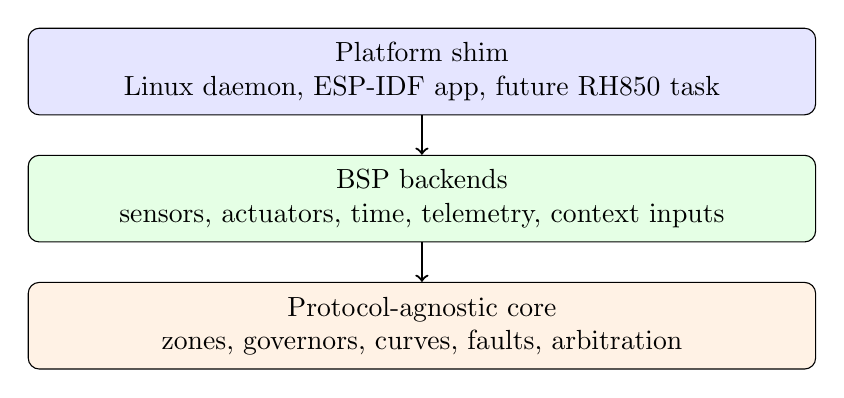
\begin{tikzpicture}[
    block/.style={rectangle, draw, rounded corners, minimum width=10cm, minimum height=1.1cm, align=center},
    arrow/.style={->, thick}
]
    \node[block, fill=blue!10] (platform) {Platform shim\\Linux daemon, ESP-IDF app, future RH850 task};
    \node[block, fill=green!10, below=0.5cm of platform] (bsp) {BSP backends\\sensors, actuators, time, telemetry, context inputs};
    \node[block, fill=orange!10, below=0.5cm of bsp] (core) {Protocol-agnostic core\\zones, governors, curves, faults, arbitration};
    \draw[arrow] (platform) -- (bsp);
    \draw[arrow] (bsp) -- (core);
\end{tikzpicture}
\caption{High-level architecture. The core does not parse platform protocols.}
\label{fig:thermal-core-architecture}
\end{figure}

\subsection{Core Boundary}

The core may depend on fixed-size configuration structures, numeric IDs, deterministic integer math, and a platform vtable. It must not depend on JSON, SocketCAN, sysfs, pthreads, ESP-IDF APIs, OBD-II encoders, or file descriptors.

\subsection{To Fill In Later}

\begin{itemize}[leftmargin=*]
    \item final public headers;
    \item memory ownership rules;
    \item exact initialization sequence;
    \item platform-specific diagrams for Linux and ESP32.
\end{itemize}

\endinput

\section{Component Design}

\subsection{Sensors}

Sensors provide temperature samples in millidegrees Celsius. Platform backends may read Linux \texttt{hwmon}, files, serial HIL input, 1-Wire probes, I2C sensors, or future automotive sensor paths. The core receives only numeric sensor IDs and typed values.

\subsection{Actuators}

The v1 actuator model is a PWM fan with optional tach feedback. The actuator definition includes minimum PWM, maximum PWM, slew limit, and stall threshold.

\subsection{Context Inputs}

Vehicle speed is the first context input. It is deliberately not special in the core: future context inputs such as ignition state, ambient temperature, HVAC state, and drive mode should use the same mechanism.

\subsection{Fault Detectors}

Initial fault detectors:

\begin{itemize}[leftmargin=*]
    \item fan stall while PWM is above a configured threshold;
    \item stuck sensor over a configured observation window;
    \item thermal runaway when temperature rises despite requested cooling;
    \item stale context input --- for example a speed-source timeout, which drives acoustic-mask fail-safe behavior.
\end{itemize}

\subsection{Numeric Identity}

Every entity the core manipulates is addressed by a small integer, never a string: sensors, actuators, zones, and context signals carry numeric IDs assigned at configuration load. Telemetry signal IDs are partitioned into fixed namespaces --- zone temperatures, actuator outputs, PID terms, context values, modifier outputs, and fault counters --- so a decoder can classify a signal from its ID alone. Fault detectors instantiate per target: one stall detector per actuator, one stuck-sensor detector per sensor, one runaway detector per zone, one stale-context detector per context signal. Each detector runs a common state machine --- normal, then degraded or critical or latched, then recovering --- with per-detector severity, action, and persistence and recovery tick counts. The exact struct layouts, enum values, and the signal-ID and event-code tables are project header artefacts and are catalogued in the appendix reference rather than transcribed here, so the paper cannot drift out of sync with the code.

\endinput

\section{Governors and Control Loop}

\subsection{Loop Overview}

The control loop is single-threaded from the core perspective. The platform calls one step function at a fixed period.

\begin{lstlisting}[language=C,caption={Conceptual control-loop order}]
thermal_core_step(ctx):
    read sensors through platform snapshot
    update filters and zone temperatures
    evaluate trips
    run each zone governor
    arbitrate shared actuators
    apply policy modifiers
    apply slew limits
    emit telemetry and fault events
\end{lstlisting}

Figure~\ref{fig:closed-loop-control} shows the same flow as a closed-loop control system. The protocol-agnostic core owns the middle of the loop: filtering, zone state, trip evaluation, governor output, arbitration, policy modifiers, slew limits, faults, and telemetry. Platform-specific code only supplies snapshots and applies actuator requests.

\begin{figure}[htbp]
\centering
\resizebox{\textwidth}{!}{%
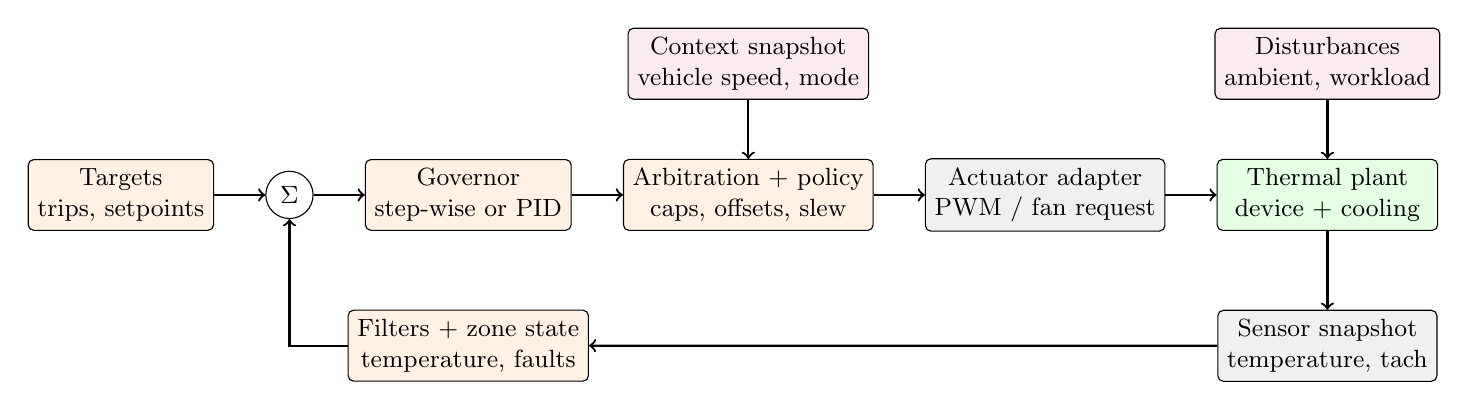
\begin{tikzpicture}[
    font=\small,
    node distance=0.72cm,
    block/.style={draw, rounded corners=2pt, align=center, minimum height=0.85cm, minimum width=2.35cm, fill=blue!6},
    coreblock/.style={block, fill=orange!10},
    ioblock/.style={block, fill=gray!12},
    plantblock/.style={block, fill=green!10, minimum width=2.8cm},
    contextblock/.style={block, fill=purple!8, minimum width=2.6cm},
    sum/.style={circle, draw, align=center, inner sep=1pt, minimum size=0.6cm, fill=white},
    arrow/.style={->, thick}
]
    \node[coreblock] (target) {Targets\\trips, setpoints};
    \node[sum, right=0.65cm of target] (compare) {$\Sigma$};
    \node[coreblock, right=0.65cm of compare] (governor) {Governor\\step-wise or PID};
    \node[coreblock, right=0.65cm of governor] (policy) {Arbitration + policy\\caps, offsets, slew};
    \node[ioblock, right=0.65cm of policy] (actuator) {Actuator adapter\\PWM / fan request};
    \node[plantblock, right=0.65cm of actuator] (plant) {Thermal plant\\device + cooling};

    \node[contextblock, above=0.75cm of policy] (context) {Context snapshot\\vehicle speed, mode};
    \node[contextblock, above=0.75cm of plant] (disturbance) {Disturbances\\ambient, workload};
    \node[ioblock, below=1.0cm of plant] (sensors) {Sensor snapshot\\temperature, tach};
    \node[coreblock, below=1.0cm of governor] (filters) {Filters + zone state\\temperature, faults};

    \draw[arrow] (target) -- (compare);
    \draw[arrow] (compare) -- (governor);
    \draw[arrow] (governor) -- (policy);
    \draw[arrow] (policy) -- (actuator);
    \draw[arrow] (actuator) -- (plant);
    \draw[arrow] (disturbance) -- (plant);
    \draw[arrow] (context) -- (policy);
    \draw[arrow] (plant) -- (sensors);
    \draw[arrow] (sensors.west) -- (filters.east);
    \draw[arrow] (filters.west) -| (compare.south);
\end{tikzpicture}%
}
\caption{Protocol-agnostic closed-loop thermal-control model}
\label{fig:closed-loop-control}
\end{figure}

\subsection{Governors}

The step-wise governor maps trip state to discrete cooling states. The PID governor targets a setpoint using Q16.16 fixed-point math by default. Anti-windup behavior and output clamping must be specified before final release.

\subsection{Arbitration}

When multiple zones request the same actuator, v1 uses max-wins arbitration. This is conservative and easy to reason about for a single shared fan.

\subsection{To Fill In Later}

\begin{itemize}[leftmargin=*]
    \item final pseudocode matching implementation order;
    \item fixed-point PID equations;
    \item anti-windup rule;
    \item unit-test references for step-wise and PID behavior.
\end{itemize}

\endinput

\section{Configuration Format}

\subsection{Linux JSON}

Linux loads JSON at startup and converts it into the same static configuration shape used by MCU targets. JSON is a platform convenience, not a core dependency.

\begin{lstlisting}[caption={Top-level configuration sketch}]
{
  "control_period_ms": 100,
  "sensors": [],
  "actuators": [],
  "zones": [],
  "policy_modifiers": [],
  "fault_detection": {},
  "telemetry": {}
}
\end{lstlisting}

\subsection{MCU Static Configuration}

Embedded builds use a generated or hand-written \texttt{static const thermal\_config\_t}. The JSON parser is not linked into MCU firmware.

\subsection{Validation}

Configuration validation should reject duplicate IDs, references to missing sensors or actuators, zones without sensors, out-of-bounds curve points, invalid PWM limits, and unsupported governor or policy names.

\subsection{To Fill In Later}

Add the final JSON Schema path, a complete bench config, and a generated static C example.

\endinput

\section{Telemetry, Runtime Tuning, and Scenarios}

\subsection{Telemetry}

The core emits numeric telemetry tuples through the platform vtable. Platforms decide whether those tuples are sent over UDP, USB-CDC, UART, CAN, or written as CSV.

\begin{lstlisting}[caption={Telemetry frame sketch}]
u32 timestamp_ms
u16 signal_id
u16 reserved
i32 value
\end{lstlisting}

\subsection{Runtime Tuning}

Runtime tuning is a bench and development feature. Commands may adjust PID gains, setpoints, trip points, curve points, and fault injection state, but all values remain bounded by compile-time or configuration limits.

\subsection{Scenario Runner}

Scenario files should make benchmark runs reproducible. For speed-aware scenarios, the runner may command \texttt{car-can-emulator} over TCP while \texttt{thermal-core} observes only CAN traffic.

\subsection{To Fill In Later}

\begin{itemize}[leftmargin=*]
    \item final command frame format;
    \item \texttt{thermalcore-probe} CLI examples;
    \item \texttt{thermalcore-tune} CLI examples;
    \item first three canonical scenario files.
\end{itemize}

\endinput

\section{Build, Deployment, and HIL Setup}\label{sec:deployment}

\subsection{Linux Daemon}

The Linux reference binary is \texttt{thermalcored}. \texttt{make build} produces it under \texttt{build/platform-linux/}; it loads a JSON configuration, binds platform backends (\texttt{hwmon} or file sensors, \texttt{sysfs} or HIL PWM, SocketCAN context), starts the configured telemetry transport, and calls \texttt{thermal\_core\_step()} once per control period:

\begin{lstlisting}[caption={Running the Linux daemon}]
make build
build/platform-linux/thermalcored --config=my-config.json
\end{lstlisting}

The same daemon serves all three Linux roles --- a standalone Raspberry~Pi~4 regulator, the scenario-clock host for the determinism harness, and the host side of the hardware-in-the-loop setup --- selected entirely by configuration.

\subsection{ESP32-C3 Firmware: Three Build Modes}

The reference firmware targets the ESP32-C3 and links the same portable \texttt{core/} and \texttt{protocol/} C99 sources as the Linux daemon. It builds in three mutually exclusive modes, selected by a CMake flag (the build system rejects any attempt to enable two at once):

\begin{table}[h]
\centering
\begin{tabular}{p{0.26\textwidth}p{0.62\textwidth}}
\toprule
\textbf{Mode} & \textbf{Behavior} \\
\midrule
\texttt{STANDALONE} (default) & The ESP32 reads its DS18B20 probe and fan tachometer, runs \texttt{thermal\_core\_step()} locally, drives the fan over LEDC PWM, and prints a human-readable status line. \\
\texttt{REPLAY\_STANDALONE} & Synthetic input snapshots baked into \texttt{.rodata} replace the live sensors; the core runs locally and emits a byte-stable CSV. Used for on-target determinism checks without any wiring. \\
\texttt{HIL\_PERIPHERAL} & The ESP32 owns only the peripherals; the Linux daemon runs the core. See below. \\
\bottomrule
\end{tabular}
\caption{ESP32-C3 firmware build modes.}
\label{tab:esp32-modes}
\end{table}

\begin{lstlisting}[caption={Building and flashing the firmware}]
cd platform/esp32_idf
idf.py build                                  # STANDALONE
idf.py -DTHERMALCORE_REPLAY_STANDALONE=ON build
idf.py -DTHERMALCORE_HIL_PERIPHERAL=ON  build
idf.py flash monitor                           # flash + serial console

# all three modes + size-budget check, from the repo root:
make build-esp32
\end{lstlisting}

\subsection{Hardware-in-the-Loop}

\texttt{HIL\_PERIPHERAL} mode splits the system across the USB cable. The ESP32-C3 owns the board-support layer --- DS18B20 over 1-Wire, the tachometer GPIO interrupt, LEDC PWM --- and nothing else. It samples the peripherals, encodes each reading as a \texttt{TELEM\_SAMPLE} \texttt{TC} frame, and streams it over USB-Serial-JTAG to the Linux daemon. The daemon runs \texttt{thermal\_core\_step()}, then sends the resulting fan duty back as a \texttt{CMD\_REQUEST} frame, which the firmware applies to the PWM output. The control law executes on the host while the real sensor and the real fan stay on the bench.

Because both ends link the identical \texttt{core/} source, HIL is also a portability check: a control decision computed by the Linux daemon over HIL is the decision the \texttt{STANDALONE} firmware would have computed on the same inputs. A bench bring-up of this loop is reported in Section~\ref{sec:evaluation}.

\subsection{OBD-II Emulator}

\texttt{car-can-emulator} is included as a submodule under \texttt{tools/car-can-emulator/} and tracks the upstream \texttt{v2-improvements} branch. It is a test dependency, not a runtime dependency of the thermal core: it synthesizes OBD-II vehicle-speed responses on a virtual CAN interface so the acoustic-mask policy and the CAN fault paths can be exercised in CI without a vehicle.

\begin{lstlisting}[caption={Emulator build}]
git submodule update --init --recursive
cmake -H tools/car-can-emulator -B build/car-can-emulator
cmake --build build/car-can-emulator
\end{lstlisting}

\subsection{Step-by-Step Guides}

The repository carries three task-oriented guides under \texttt{docs/getting-started/} that walk through each deployment with exact wiring and commands: \texttt{esp32-standalone.md} (a self-contained ESP32-C3 regulator), \texttt{linux-pi4.md} (a Raspberry~Pi~4 daemon driving a \texttt{sysfs} PWM fan), and \texttt{hil-peripheral.md} (the ESP32-plus-daemon HIL loop). This section gives the architecture; those guides give the keystrokes.

\endinput

\section{Summary, Limitations, and Future Work}

\subsection{Summary}

This document describes a protocol-agnostic thermal-control core that has been implemented and exercised across a Linux host and the ESP32-C3, including a hardware-in-the-loop bring-up in which the host runs the control law over real bench peripherals. The implementation through Stage~14 is complete and CI-gated; the formal cross-platform benchmark sweep that will close the evidence trail is still pending. The result is not a production safety component, but a reproducible reference design with a measured-only evidence trail (Section~\ref{sec:evaluation}).

\subsection{Known Limitations}

\begin{itemize}[leftmargin=*]
    \item not ASIL-rated;
    \item no AUTOSAR integration in v1;
    \item OBD-II speed is a reproducible test source, not a production IVI integration strategy;
    \item PWM-seconds is only an acoustic proxy;
    \item RH850 is structurally planned but not hardware-validated in v1;
    \item the formal timing and acoustic benchmarks are not yet captured (Section~\ref{sec:eval-gaps}).
\end{itemize}

\subsection{Future Work}

\begin{itemize}[leftmargin=*]
    \item calibrated SPL measurement;
    \item multi-input policy modifiers;
    \item OEM CAN DBC integration outside the core;
    \item PID autotune;
    \item full RH850 validation;
    \item static-analysis and MISRA-oriented hardening.
\end{itemize}

\subsection{Draft Status}

The conceptual and implementation sections of this draft are written against the shipped code. The Evaluation section is preliminary: it will grow from the measured footprint, determinism, and bring-up results reported here to the full benchmark sweep --- with regenerated figures --- once that pipeline lands. Final quantitative claims and practical recommendations are written at that point.

\endinput


\clearpage

%------------------------
% Appendices
%------------------------
\section{Appendix A: Units and Numeric Conventions}

\begin{table}[h]
\centering
\begin{tabular}{lll}
\toprule
\textbf{Quantity} & \textbf{Unit} & \textbf{Representation} \\
\midrule
Temperature & millidegrees Celsius & \texttt{int32\_t} \\
PWM duty & 0--255 & \texttt{uint8\_t} \\
Fan speed & RPM & \texttt{uint16\_t} \\
Vehicle speed & km/h & \texttt{uint16\_t} \\
Time & milliseconds & \texttt{uint32\_t}, rollover-aware \\
PID gains & Q16.16 & \texttt{int32\_t} \\
\bottomrule
\end{tabular}
\caption{Numeric conventions to keep consistent across code and paper.}
\end{table}

\section{Appendix B: OBD-II Speed Reference}

The reference speed source is OBD-II Service 01 PID \texttt{0x0D}. \texttt{thermal-core} does not parse this inside the core; Linux and ESP32 platform code decode the CAN response and expose typed speed to the core.

\begin{itemize}[leftmargin=*]
    \item Request IDs: \texttt{0x7DF} and \texttt{0x7E0}
    \item Response ID: \texttt{0x7E8}
    \item Response mode: \texttt{0x41}
    \item PID: \texttt{0x0D}
    \item Value: one byte, direct km/h
\end{itemize}

\section{Appendix C: Benchmark Matrix}

\begin{table}[h]
\centering
\begin{tabular}{p{0.28\textwidth}p{0.52\textwidth}}
\toprule
\textbf{Scenario} & \textbf{What to report} \\
\midrule
\texttt{idle\_steady\_state} & false faults, fan off behavior \\
\texttt{heat\_soak\_ramp} & PWM response, maximum temperature \\
\texttt{step\_load} & settling time, overshoot \\
\texttt{fan\_stall\_recovery} & stall detection and recovery latency \\
\texttt{acoustic\_mask\_high\_speed} & cap release and trip offset behavior \\
\texttt{can\_bus\_loss} & timeout and fail-safe behavior \\
\bottomrule
\end{tabular}
\caption{Initial benchmark matrix. Add CSV filenames and git SHA values later.}
\end{table}

\section{Appendix D: Fill-In Checklist}

\begin{itemize}[leftmargin=*]
    \item final BOM and wiring diagram;
    \item complete JSON configuration;
    \item generated static MCU configuration;
    \item telemetry signal table;
    \item numeric event code table;
    \item exact build and flash commands;
    \item benchmark raw-data paths;
    \item figure regeneration commands.
\end{itemize}

\endinput


\end{document}
